%%

\section{FLOSS business models}

\subsection{Introduction}

\begin{frame}
\frametitle{The million dollar question}

Once upon a time, the key question for companies/projects/individuals entering the
FLOSS universe was:

\begin{itemize}
 \item \textit{How can we make money with FLOSS?}
\end{itemize}

\pause
But now, the question is

\begin{itemize}
\item \textit{Which are the most successful business strategies that we can adopt around FLOSS?}
\end{itemize}
\end{frame}

\begin{frame}
 \frametitle{Origin: open innovation}
 \begin{itemize}
  \item Some (few) people are still against the added-value provided by knowledge aperture (source
code is just an example).
  \item Case study: \textbf{GoldCorp} \texttt{http://www.goldcorp.com/}
    \begin{itemize}
    \item Traditional mining company, needs to find new veins.
    \item Executive President Rob McEwen publishes open contest (2000): 575K\$ for participants
    who offer best methods to choose new extraction points.
    \item 80\% of answers produced positive results.
    \item 100\$ invested in 1993 is worth over 3.000\$ in 2005.
    \end{itemize}
  \item However, \textbf{crowdsourcing is orthogonal to libre software}
 \end{itemize}
\end{frame}

\begin{frame}
 \frametitle{Current trends}
 \begin{itemize}
 \item ``\textit{There is no silver bullet}''
 \item Every company/project/individual should select appropriate strategies for their particular needs.
 \item And being alert to change/evolve their model on the fly, in response to rapid changes in the market
and surrounding conditions.
 \item Luckly, there exist \textbf{many} options to choose from.
 \end{itemize}
\end{frame}

\begin{frame}
 \frametitle{False myths}
\begin{itemize}
 \item Many companies justify the cost of proprietary software with the economic cost of production (development) process.
\item Two types of product value:
    \begin{itemize}
     \item \alert{Use} value: Economic value as a tool, productivity growth (value as an intermediate good).
     \item \alert{Sale} value: Value as a market product (value as a final product).
    \end{itemize}
\item Aprox. 75\% of salaried programmers work is devoted to
\alert{maintenance} tasks, not to \alert{development} of new features.
\end{itemize}

\end{frame}

\begin{frame}
 \frametitle{False myths}
\begin{itemize}
 \item Contrary to other products, the true \alert{value} of software does not lie in its production
or replacement cost (food, cars, engines, appliances...).
 \item The upper limit of the value of software for clients is imposed by 
the \alert{expected value} of the future \alert{service} that sellers offer to clients.
      \begin{itemize}
       \item Software stability.
       \item Help-desk, support services.
       \item Documentation.
       \item Software customization.
       \item Training and certification.
      \end{itemize}
  \pause
  \centering{\alert{services == source of revenues}}
\end{itemize}

\end{frame}

\begin{frame}
 \frametitle{False myths}
\begin{itemize}
 \item The organizational model of libre software allows to provide services in a more profitable,
scalable and sustainable way.
\begin{itemize}
 \item \alert{Users} become \alert{clients}.
 \item \alert{Scalability} in failures identification and solution.
 \item \alert{Sharing risks} and production \alert{costs}.
 \item Monopolistic practices made \alert{difficult}.
\end{itemize}
\end{itemize}

\end{frame}

\begin{frame}
 \frametitle{False myths}
\begin{itemize}
 \item Myth: ``The Commons tragedy''.
 \item Any business model would be doomed to fail, or else, to result 
in a new scenario with closed solutions.
 \item Antidote: In fact \alert{software use} does not \alert{reduce} but it
\alert{increments its value}.
    \begin{itemize}
    \item Larger user community (potential clients).
    \item Benefit from patches and proposed solutions.
    \item Benefit from new features.
    \item Contributing to leverage product quality (guarantee absence of conflicts 
with business interests).
    \end{itemize}
\centering{\alert{``Inverse commons''}}
\end{itemize}
\end{frame}

\begin{frame}
 \frametitle{Central idea}
\Large{The \alert{business model} must always pivot on the \alert{use value}, not on the
sale value.}
\end{frame}

\subsection{Taxonomy of FLOSS business models}

%\subsection{FLOSS: A guide for SMEs}

\begin{frame}
 \frametitle{FLOSS: A guide for SMEs}
\begin{center}
 \begin{LARGE} FLOSS by itself is not, and it has never been, a business model. \end{LARGE}
\end{center}
\begin{center}
 Companies must desing a \alert{strategy}, create a \alert{business plan} and ensure 
\alert{securing benefits} aimed to a sustainable growth.
\end{center}
\begin{center}
 FLOSS can improve \alert{viability} and \alert{efficiency} with many business models.
\end{center}


\end{frame}

\begin{frame}
 \frametitle{FLOSS: A guide for SMEs}
 \begin{itemize}
  \item Report ellaborated for FLOSSMETRICS, EU FP6 project.
  \item Analysis of 218 companies receiving at least 25\% of their total revenues directly or indirectly from FLOSS.
  \item Identifying common business strategies around FLOSS.
  \item Recommendations about required conditions to apply each model.
 \end{itemize}
\end{frame}

\begin{frame}
 \frametitle{3 axes influencing software landscape}
 \begin{itemize}
  \item \alert{Software model}
  \begin{itemize}
   \item Proprietary vs. libre software.
  \end{itemize}
  \item \alert{Development model}.
  \begin{itemize}
   \item Barriers to collaboration.
   \item Single developer/reduced group vs. large community, global outreach.
  \end{itemize}
  \item \alert{Business model}.
  \begin{itemize}
   \item Type of revenues model.
   \item Numerous options: Training, support, on-demand changes, productizing, SaaS, etc.
  \end{itemize}
 \end{itemize}
\end{frame}

\begin{frame}
 \frametitle{Strategic uses of libre software}
 \begin{itemize}
  \item The Gartner consulting group pointed out: in 2012, use of libre software would reach 90\% of companies worldwide.
  \item Companies forced to adapt their software to work under multiple conditions.
  \item Emerging trend in big companies towards source code release under FLOSS licenses.
More active interaction with nearby projects.
  \item Proprietary software success is now guaranteed only if there are no alternative and reliable FLOSS options.
 \end{itemize}
\end{frame}


\begin{frame}
 \frametitle{Carlo Daffara taxonomy (FLOSSMETRICS)}
 \begin{itemize}
  \item \textit{Dual licensing}: FLOSS version and proprietary version.
  \item \textit{Open core}: Allows mixing FLOSS and proprietary elements.
  \item \textit{Product specialists}: Superior knowledge, additional services.
  \item \textit{Platform providers}: Integration, product testing.
  \item \textit{Aggregate support providers}: Primer nivel de soporte para diferentes
tipos de software libre.
  \end{itemize}
  \end{frame}
  
\begin{frame}
 \frametitle{Carlo Daffara taxonomy (FLOSSMETRICS)}
 \begin{itemize}
\item \textit{Selection/consulting companies}: Closer to the analyst role, minimum impact on FLOSS communities.
  \item \textit{Legal certification and consulting}: Assessment on license compatibility.
  \item \textit{Training and documentation}: Either as part of a broader support contract or companies exclusively devoted
to this market area.
  \item \textit{R\&D cost sharing}: Initial investment + creating community to reduce R\&D costs.
  \item \textit{Indirect revenues}: Baseline for sales of associated products or services (commodities).
 \end{itemize}
\end{frame}

\begin{frame}
 \frametitle{Dual (or multiple) licensing}
 \begin{itemize}
  \item Examples: MySQL (GPL+prop.), Mozilla software (MPL, GPL, LGPL).
  \item The owner of source code IPR selects a double licensing strategy.
  \begin{itemize}
   \item \textbf{Copyleft license}: To obtain some benefits (community contribution, integration in other libre software, etc.).
   \item \textbf{Proprietary license of permissive free license}: Other companies might integrate this software with
   proprietary software.
  \end{itemize}  
  \item Leverage adoption and visibility, offering solutions to proprietary software companies.
  \item But it may also limit contributions from FLOSS developers (we force them to release the ownership  of the code
  to maintain the right of dual licensing).
 \end{itemize}
\end{frame}

\begin{frame}
 \frametitle{Open core}
 \begin{itemize}
  \item Also based on dual licensing, but this is not the business foundation.
  \item Examples: SugarCRM, SendMail.
  \item Different features linked to licenses:
  \begin{itemize}
   \item \textbf{Libre core}: Basic version of the software, including minimal working functinalities,
   is libre software.
   \item \textbf{Proprietary added-value functionalities}: Most sophisticated features, targeting the
   enterprise sector and expert audience, are released under proprietary license.
  \end{itemize}  
  \item Revenues concentrate on commercialization of proprietary components, plus support and
  extension/customization.
  \item FLOSS developers might distrust the project, for the same reasons as dual licensing.
 \end{itemize}
\end{frame}

\begin{frame}
 \frametitle{Product specialists}
 \begin{itemize}
  \item Company offering or creating maintainance for a specific software product, usually in a concrete market.
  \item Example: Alfresco (Content Management System).
  \item Main revenues come from training, consulting, specialized support for installation, deployment and
  configuration, extensions, customization, etc.
  \item Typical model ``best product knowledge here'' or ``best source code here''.
  \item It is mandatory to retain the best team of specialists.
  \item High risk of other competitors entering at the same level of knowledge and specialization in the same
  market.
 \end{itemize}
\end{frame}

\begin{frame}
 \frametitle{Platform providers}
 \begin{itemize}
  \item Selection, support, integration and services around a set of projects integrated in a single, tested
and verified product.
  \item Key points:
  \begin{itemize}
   \item Verification process to meet quality standards.
   \item Additional services (support, training, customization).
  \end{itemize}
  \item Copyright ownership prevents direct copy (not cloning).
  \item Example: RedHat.
  \item The source code is libre software, but the product name and logo are trademarks.
  \item Considerable effort to eliminate them from files, documentation, etc.
 \end{itemize}
\end{frame}

\begin{frame}
 \frametitle{Aggregate support providers}
 \begin{itemize}
  \item Centralized support point for different libre software products.
  \item Two strategies:
  \begin{itemize}
   \item Employing developers specialized in those products.
   \item Redirecting petitions to other support specialists.
  \end{itemize}
  \item Clear benefit for large projects whose costs could raise due to excessive
diversification of support channels (comprehensive help-desk).
  \item It only works for clients with many different products running on mission-critical platforms.
  They assure exclusive support contracts.
  \item Example: OpenLogic.
 \end{itemize}
\end{frame}

\begin{frame}
 \frametitle{Selection/consulting companies}
 \begin{itemize}
  \item Usually, they do not develop software.
  \item Assessment about selection and evaluation of software products and services.
  \item It might save costs for clients (software selection process can add up to 45\% of
total costs of software adoption).
  \item Experience to undertake selection process is not easily replicable.
  \item Sometimes, they develop dedicated tools aimed for selection, that they do not release as
free software to stop competence.
  \item Example: Open WebApps.
 \end{itemize}
\end{frame}

\begin{frame}
 \frametitle{Legal certification/consulting}
 \begin{itemize}
  \item They do not usually develop software, either.
  \item Legal assessment for companies about complex problems derived from multiplicity of libre software
licenses and their compatibilities.
  \item They might save costs for integrators less familiarized with selection process and licensing checking.
  \item Example: Palamida.
 \end{itemize}
\end{frame}

\begin{frame}
 \frametitle{Training and documentation}
 \begin{itemize}
  \item Focused on important aspects of libre software, but not directly related to development.
  \begin{itemize}
   \item Training users and tech staff.
   \item Support for certification processes (technical staff and end-users).
   \item Creation of high quality documentation.
  \end{itemize}
  \item It is very helpful if supported products have a large user base (size of target market).
  \item Certification programs might provide extra income, conditions for collaboration agreements
(partnerships).
  \item Example: Gbdirect.
 \end{itemize}
\end{frame}

\begin{frame}
 \frametitle{R\&D cost sharing}
 \begin{itemize}
  \item Company interested in software development decides to release the code to benefit from
contributions from large community of interested developers.
  \item Development cost of closed source alternative would be prohibitive.
  \item Viability conditions:
  \begin{itemize}
   \item Great branding and public image to attract attention from stakeholders.
   \item Solvency to develop and nurture community participation.
   \item Investment in project support (IDE, events, promotion, etc.).
  \end{itemize}
   \item Example: Maemo (Nokia).
 \end{itemize}
\end{frame}

\begin{frame}
 \frametitle{Indirect revenues}
 \begin{itemize}
  \item Companies that decide to develop libre software or funding libre software projects to leverage
their business on related products.
  \item Some examples:
   \begin{itemize}
    \item Hardware makers: Intel, Dell. Broaden their target audience base providing better support for libre
software platforms.
    \item Tech books publishers: O'Reilly (contributes to Perl community, and it is the main publisher of Perl books).
   \end{itemize}
   \item Stakeholders that indirectly benefit from success of libre software projects.
 \end{itemize}
\end{frame}

\begin{frame}
\frametitle{Distribution of models identified in the study}
\begin{figure}
 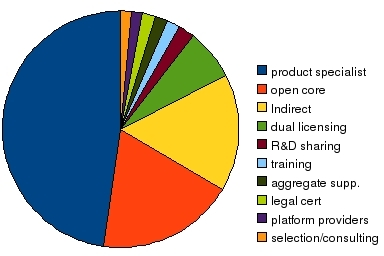
\includegraphics[height=4cm]{figs/models-share.jpg}
\end{figure}
\end{frame}

\begin{frame}
\frametitle{Evolution CAGR in FLOSS business}
\begin{center}
\begin{figure}
 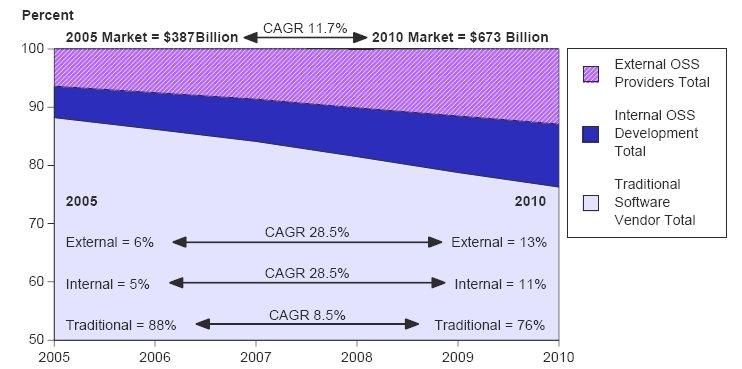
\includegraphics[height=4.5cm]{figs/Economic-Gartner.jpg}
 \caption{\small Taken from ``Open Source going mainstream'', Gartner group report.}
\end{figure}
\end{center}
\end{frame}

\begin{frame}
\frametitle{Companies running business around FLOSS (selection)}
\begin{center}
\begin{figure}
 
\includegraphics[height=4.5cm]{figs/floss-companies.jpg}
 \caption{\small Taken from ``FLOSS: A guide for SMEs'', Carlo Daffara (FLOSSMETRICS EU FP6)}
\end{figure}
\end{center}
\end{frame}



% \subsection{Clasificación extendida}
% \begin{frame}
%  \frametitle{Alternativas de modelos de negocio (extendida)}
%  \begin{itemize}
%   \item Con financiación externa
%   \begin{itemize}
%    \item El fundador generalmente decide cómo y dónde gastar los recursos.
%    \item Orientado hacia la producción de software.
%    \item En cierto modo, es una estrategia de esponsorización.
%   \end{itemize}
%   \item Auto-financiados
%   \begin{itemize}
%    \item Ingresos de las actividades de la compañía.
%    \item Puede haber desarrollo de software o no.
%   \end{itemize}
%   \item Desarrollado sin financiación directa.
%   \item Desarrollado para uso interno.
%   \item Modelos mixtos.
%  \end{itemize}
% \end{frame}
% 
% \begin{frame}
%  \frametitle{Financiación externa}
%  \textbf{Financiación pública}
%  \begin{itemize}
%   \item Similar a proyectos de I+D.
%   \item Financiación puede venir de instituciones que promuevan I+D.
%   \item Institución financiadora normalmente no busca beneficios directos.
%   \item Expresamente realizada sólo en casos particulares; principalmente como 
% ``subproducto`` de un contrato.
%  \end{itemize}
% \end{frame}
% 
% \begin{frame}
%  \frametitle{Negocios con financiación externa}
%  \textbf{Financiación externa (motivaciones y casos de estudio)}
%  \begin{itemize}
%   \item ``Científica'': Software requerido para producir resultados
% que deben estar disponibles, para publicación científica.
%   \item ``Pre-competitive'': Beneficios industriales de resultados pre-competitivos.
%   \item ``Promoción de estandar'': Implementación de referencia o estándar (probablemente, la
% norma o estándar también abierta).
%   \item `Motivación social'': Financiación de infraestructura básica para la Sociedad de la Información.
%   \item  Caso de estudio: Gnat (compilador de Ada), alrededor de 1 M\$ del Gobierno Federal EE.UU.
% a la NYU para su desarrollo.
%   \end{itemize}
% \end{frame}
% 
% \begin{frame}
%  \frametitle{Negocios con financiación externa}
%  \textbf{Fianciación privada sin ánimo de lucro}
%  \begin{itemize}
%   \item Normalmente, proviene de de ONGs y fundaciones privadas.
%   \item Motivación ``directa'': Producción de software libre.
%   \item Motivación ``indirecta'': Contribuye a resolver el problema de creación de solución software.
%   \item En general, mecanismos similares a la financiación pública.
%   \item Casos de estudio:
%   \begin{itemize}
%    \item Free Software Foundation
%    \item Open Bioinformatics Foundation
%   \end{itemize}
%  \end{itemize}
%  \hfill \large \texttt{http://fsf.org}\\
%  \hfill \large \texttt{http://open-bio.org}
% \end{frame}
% 
% \begin{frame}
%  \frametitle{Negocios con financiación externa}
%  \textbf{Financiación de fuentes interesadas en mejoras}
%  \begin{itemize}
%   \item Alguien necesita mejoras en un producto de sofware libre.
%   \item Desarrollo financiado por un grupo o compañía.
%   \item Caso de estudio:
%   \begin{itemize}
%    \item Corel quería tener una versión de sus productos para GNU/Linux.
%    \item Wine podía contribuir a ahorrar costes si se mejoraba.
%    \item Corel financió contribuciones de Macadian para Wine, incluyendo las que
% ellos mismos necesitaban.
%   \end{itemize}
%   \hfill \large \texttt{http://www.macadamian.com/news/wine.html}
%  \end{itemize}
% \end{frame}
% 
% \begin{frame}
%  \frametitle{Negocios con financiación externa}
%  \textbf{Financiación indirecta}
%  \begin{itemize}
%   \item Financiación de desarrollo de software a través de beneficios obtenidos mediante productos
% relacionados.
%   \item Normalmente, las ventajas (incluyendo aquellas que se ponen a la venta) no son exclusivas.
%   \item Ventajas mejores cuanto mayor es el porcentaje de mercado en ese nicho.
%   \item Ejemplos: libros, hardware, distribuciones.
%   \begin{itemize}
%    \item O'Reilly financia el desarrollo de Perl development, y es la principal editorial que publica
% sobre este tema.
%    \item RedHat financia desarrollo GNOME para garantizar un escritorio fiable para su propia distribución.
%    \end{itemize}
%  \end{itemize}
%   \hfill \large \texttt{http://oreilly.com}\\
%   \hfill \large \texttt{http://redhat.com}
% \end{frame}
% 
% \begin{frame}
%  \frametitle{Modelos de negocio auto-financiados}
%  \textbf{Basados en un conocimiento superior}
%  \begin{itemize}
%   \item Venta de servicios basada en un mejor conocimiento del producto.
%   \item Conocimiento es principalmente adquirido trabajando en el proyecto y colaborando en su desarrollo.
%   \item Desarrollo del producto también ayuda por motivos de imagen.
%   \item Pero la participación en el desarrollo no es obligatoria.
%   \item Normalmente se vende servicios de consultoría, adaptación, integración, etc.
%  \end{itemize}
% \end{frame}
% 
% \begin{frame}
%  \frametitle{Modelos de negocio auto-financiados}
%  \textbf{Basados en un conocimiento superior pero con limitaciones}
%  \begin{itemize}
%   \item Estos modelos tratan de limitar el efecto de compañías competidoras.
%   \item Típicamente se emplean patentes o licencias propietarias.
%   \item Normalmente, estos mecansimos se aplican en partes pequeñas pero fundamentales del 
% producto desarrollado.
%   \item En la mayoría de casos, la comunidad de software libre desarrolla su propia versión de
% estos componentes.
%  \end{itemize}
% \end{frame}
% 
% \begin{frame}
%  \frametitle{Modelos de negocio auto-finaciados}
%  \textbf{Basados en ser la fuente de un programa}
%  \begin{itemize}
%   \item Similar a aquellos basados en un conocimiento superior.
%   \item Ventaja competitiva obtenida de convertirse en desarrolladores de un
% producto, y tenerlo listo antes que la competencia.
%   \item Muy interesante en términos de imagen.
%   \item Casos de estudio:
%   \begin{itemize}
%    \item Evolution, RedCarpet (Ximian, hoy Novell).
%    \item Zope (Zope Corporation, anteriormente Digital Creations).
%   \end{itemize}
%  \end{itemize}
%  \hfill \large \texttt{http://ximian.com}\\
%  \hfill \large \texttt{http://zope.com}
% \end{frame}
% 
% \begin{frame}
%  \frametitle{Modelos de negocio auto-finaciados}
%  \textbf{Basado en ser la fuente de un programa pero con limitaciones}
%  \begin{itemize}
%   \item Como en el anterior, pero imponiendo algunas limitaciones para excluir a compañías
% competidoras del proceso.
%   \begin{itemize}
%    \item Ejemplo: distribución propietaria durante un tiempo, luego libre
%    \item Ejemplo: distribución limitada durante un tiempo
%   \end{itemize}
%   \item Estos modelos se benefician menos de las ventajas del software libre; al menos desde
% el punto de vista de desarrollo (son menos cooperativos).
%   \item Casos de estudio:
%   \begin{itemize}
%    \item Alladin Ghostscript (un año entre la versión AFPL y la versión GPL).
%    \item Gnat (AdaCore) (versiones en desarrollo sólo para algunos clientes).
%   \end{itemize}
%  \end{itemize}
%  \hfill \large \texttt{http://www.ghostscript.com} 
%  \hfill \large \texttt{http://www.alladin.com}\\
%  \hfill \large \texttt{http://adacore.com}
% \end{frame}
% 
% \begin{frame}
%  \frametitle{Modelos de negocio auto-finaciados}
%  \textbf{Basados en licencias especiales}
%  \begin{itemize}
%   \item Con frecuencia, se basan en la distribución del software bajo dos o más licencias
% diferentes.
%   \item En general, se complementan con labores de consultoría de producto.
%   \item Ejemplos: Distribuciones libres bajo GPL, versiones propietarias para clientes con necesidades
% adicionales/especiales.
%   \item Caso de estudio:
%   \begin{itemize}
%    \item MySQL: \textit{Community} distribuída bajo GPL; \textit{Enterprise}, 
%    versión propietaria directamente soportada por la empresa MySQL AB, con muchas mejoras de valor añadido.
%   \end{itemize}
%  \end{itemize}
%   \hfill \large \texttt{http://mysql.com}
% \end{frame}
% 
% \begin{frame}
%  \frametitle{Modelos de negocio auto-finaciados}
%  \textbf{Basados en la venta de una marca registrada}
%  \begin{itemize}
%   \item Si el nombre gana popularidad, se puede usar para vender casi cualquier cosa.
%   \item Ejemplo: Distribuciones GNU/Linux que venden otros productos/servicios.
%   \item Caso de estudio:
%   \begin{itemize}
%    \item RedHat: Empezó inicialmente vendiendo su distribución, hoy día tiene otros núcleos clave
% de negocio como consultoría, formación, certificación, etc.
%   \end{itemize}
%  \end{itemize}
%  \hfill \large \texttt{http://www.redhat.com}
% \end{frame}
% 
% \begin{frame}
%  \frametitle{Desarrollos sin financiación directa}
%  \begin{itemize}
%   \item La mayoría de los proyectos se desarrollan fundamentalmente de este modo.
%   \item En muchos casos, tenemos ``financiación indirecta'':
%   \begin{itemize}
%    \item Compañías que permiten que sus empleados empleen parte de su tiempo para contribuir
% a software libre.
%    \item Contribuciones de organizaciones que desean cierta funcionalidad.
%    \item Contribución de infraestructuras al proyecto.
%    \item Donaciones.
%   \end{itemize}
%  \end{itemize}
% \end{frame}
% 
% \begin{frame}
%  \frametitle{Desarrollo sin financiación directa}
%   \textbf{Casos de estudio}
%  \begin{itemize}
%   \item Muchos de los grandes proyectos han establecido fundaciones que proporcionan
% cobertura legal y (parcialmente) económica.
%   \begin{itemize}
%    \item Apache Software Foundation
%    \item Gnome Foundation
%    \item KDE e. V.
%    \item Mozilla Foundation.
%    \item Plone Foundation.
%   \end{itemize}
%  \end{itemize}
%   \hfill \large \texttt{http://apache.org}\\
%   \hfill \large \texttt{http://foundation.gnome.org}\\
%   \hfill \large \texttt{http://www.kde.org/areas/kde-ev/}\\
%   \hfill \large \texttt{http://www.mozilla.org/foundation}\\
%   \hfill \large \texttt{http://plone.org/foundation}
% \end{frame}
% 
% \begin{frame}
%  \frametitle{Desarrollos internos}
%  \begin{itemize}
%   \item Al menos en su fase inicial, el producto es sólo para uso interno.
%   \item Los desarrolloadores se benefician del modelo del software libre: contribuciones, informes
% de error, parches, etc.
%   \item Las compañías obtienen beneficios también: continuidad en el soporte, inspección por terceras
% partes, documentación, mayor capacidad de desarrollo etc.
%   \item Si tienen aceptación en el mercado, se pueden comenzar a aplicar otros modelos de negocio.
%   \item Caso de estudio: Cisco Enterprise Print System (CEPS)
%  \end{itemize}
%    \hfill \large \texttt{http://ceps.sourceforge.net}
% \end{frame}
% 
% \begin{frame}
%  \frametitle{Modelos mixtos}
%  \begin{itemize}
%   \item Casi todas las compañías los usan.
%   \item Medidas para fortalecer la imagen de marca.
%   \item Pueden o no contribuir al desarrollo del software.
%   \item En casos raros, estas compañías trabajan exclusivamente con SL.
%   \item Muchas compañías ``tradicionales`` intentan nuevas opciones con el
% software libre.
%   software.
%  \end{itemize}
% \end{frame}
% 
% \subsection{Taxonomía de Hecker}
% \begin{frame}
%  \frametitle{Taxonomía de Frank Hecker (OSI)}
%  \begin{itemize}
%   \item \textit{Soporte de venta}: Venta de servicios relacionados con el producto.
%   \item \textit{Líder de pérdidas}: Venta de otros productos propietarios.
%   \item \textit{Widget frosting}: Promoción de ventas hardware.
%   \item \textit{Accesorización}: Habilitar ventas de productos físicos (libros, etc.).
%   \item \textit{Facilitador de servicios}: Servicios on-line accesibles a través del programa.
%   \item \textit{Véndelo, libéralo}: Versión cíclica del líder de pérdidas.
%   \item \textit{Licencia de marca}: Venta de royalties de marca
%   \item \textit{Franquicia de software}: Franquicia de marca.
%  \end{itemize}
% \end{frame}
% 
% \begin{frame}
%  \frametitle{Recomendaciones para migración de código a software libre}
%  \begin{itemize}
%   \item Compartición de código: Separación clara del código fuente de liberías o módulos que sean
% propietarios.
%   \item Tecnología de terceras partes: Inspeccionar el uso de librerías de terceras partes para evitar
% problemas de licencias.
%   \item Saneamiento de código: Limpieza y preparación de código fuente para contribuciones por parte de
% desarrolladores externos.
%   \item Control de expotación: Consideración de condiciones especiales de exportación de algoritmos criptográficos
% y protocolos y sistemas de seguridad (lista reducida de países fuera de EE.UU.).
%   \item Proceso de desarrollo de producto: Adaptación deprocesos de trabajo internos a nuevas contribuciones.
%  \end{itemize}
% \end{frame}

% %%%%%%%%%%%%%%%%%%%%%%%%%%%%%%%%%%%%%%%%%%%%%%%%%%%%%%%%
% 
\subsection{Conclusions}

\begin{frame}
 \frametitle{New ways of collaboration}
 \begin{itemize}
  \item Libre software can be adopted as a mean to facilitate new ways of collaboration
among different companies. \textit{Coopetition}.
  \item Several possibilities (collaboration without formal contracts or agreements).
  \item Creating business ecosystems.
  \item Empowering business opportunities.
  \item Inspiration for new applications of information sharing.
 \end{itemize}
\end{frame}

% \begin{frame}
%  \frametitle{Algunos ejemplos interesantes}
%  \begin{itemize}
%   \item AdaCore (antes ACT y ACT Europe).
%   \item Matra Datavision y OpenCascade.
%   \item Sun, StarOffice y OpenOffice.org (ahora Oracle).
%  \end{itemize}
% \hfill \large \texttt{http://www.adacore.com/}\\
% \hfill \large \texttt{http://libre.act-europe.fr/}\\
% \hfill \large \texttt{http://www.opencascade.org/}\\
% \hfill \large \texttt{http://www.opencascade.com/}\\
% \hfill \large \texttt{http://staroffice.com}\\
% \hfill \large \texttt{http://openoffice.org}
% \end{frame}

\begin{frame}
 \frametitle{References}
 \begin{itemize}
  \item ``FLOSS: A guide for SMEs''.
\texttt{http://guide.conecta.it/index.php/Main\_Page}
  \item ``The Magic Cauldron'', Eric Raymond.
  \item ``State of Open Source'', Gartner Group, 2008.
\texttt{http://arstechnica.com/open-source/news/2008/02/}
\texttt{gartner-80-percent-of-commercial-software-}
\texttt{programs-will-include-open-source-by-2012.ars}
  \item The rejuvenetion of community controlled open source.
\texttt{http://blogs.the451group.com/opensource/2009/10/15/}
\texttt{the-rejuvenation-of-community-controlled-open-source/}
 \end{itemize}

\end{frame}

% \begin{frame}
%  \frametitle{Referencias}
%  \begin{itemize}
%   \item ``Free Software, Open Source: Information Society Opportunities
%   for Europe?'', European Working Group on Libre Software.
%   \item ``Setting Up Shop'', Franck Hecker.
%   \item ``Open Source Software'', Naomi Hoffman.
%   \item ``Open Source Case for Business'', OSI.
%   \item ``The Magic Cauldron'', Eric Raymond.
%   \item ``The Wall Street Performer Protocol'', Chris Rasch.
%  \end{itemize}
% 
% \end{frame}

% \begin{frame}
%  \frametitle{Referencias}
%  \begin{itemize}
%   \item \small{\hfill  \texttt{http://eu.conecta.it}}\\
%   \item \small{\hfill  \texttt{http://www.hecker.org/writings/setting-up-shop.html}}\\
%   \item \small{\hfill  \texttt{http://public.kitware.com/VTK/pdf/oss.pdf}}
%   \item \small{\hfill  \texttt{http://www.opensource.org/advocacy/case\_for\_business.html}}\\
%   \item \small{\hfill  \texttt{http://www.tuxedo.org/~esr/writings/magic-cauldron/}}
%   \item \small{\hfill  \texttt{http://firstmonday.dk/issues/issue6\_6/rasch/index.html}}
%  \end{itemize}
% 
% \end{frame}

